\tikzstyle{level 1}=[level distance=2cm, sibling distance=2.5cm]
\tikzstyle{level 2}=[level distance=2cm, sibling distance=1cm]
\tikzstyle{dot} = [circle, minimum width=3pt,fill, inner sep=0pt]
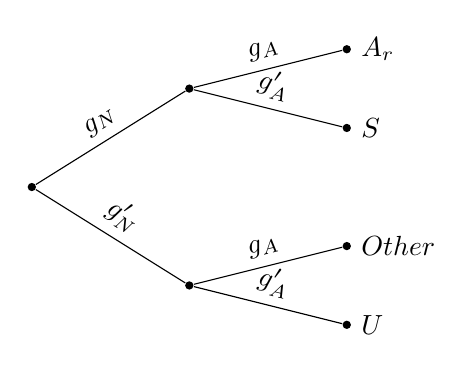
\begin{tikzpicture}[grow=right, sloped]
\node[dot]{}
    child {
        node[dot]{}
            child {
                node[dot, label=right:
                    {$U$}] {}
                edge from parent
                node[above] {$g^\prime_A$}
            }
            child {
                node[dot, label=right:
                    {$Other$}] {}
                edge from parent
                node[above] {$g_A$}
            }
            edge from parent 
            node[above] {$g^\prime_N$}
    }
    child {
        node[dot]  {}     
        child {
                node[dot, label=right:
                    {$S$}] {}
                edge from parent
                node[above] {$g^\prime_A$}
            }
            child {
                node[dot, label=right:
                    {$A_r$}] {}
                edge from parent
                node[above] {$g_A$}
            }
        edge from parent         
            node[above] {$g_N$}
    };
\end{tikzpicture}
